% !TEX program = xelatex
% Шаблон научной статьи НИТУ «МИСиС»

\documentclass{misisarticle}
\usepackage{graphicx}
\usepackage{amsmath}
\usepackage{amssymb}
\usepackage{booktabs}

% --- Классификационные коды (по ведомости МИСиС) ---
\grnti{50.09.45}
\asjc{1707, 1709}
\oecd{2.2}

% --- Название ---
\title{Сравнительный анализ качества прямых и зеркально-отражённых LiDAR-измерений при варьировании угла падения}

% --- Авторы ---
\misisauthor{Н.~Д.~Савина}{кафедра инженерной кибернетики НИТУ «МИСиС»}{Москва, Россия}{m2311397@edu.misis.ru}
\misisauthor{М.~Р.~Вишневский}{кафедра инженерной кибернетики НИТУ «МИСиС»}{Москва, Россия}{}

% --- Аннотация и ключевые слова ---
\abstract{%
Применение беспилотных летательных аппаратов (БПЛА) и мобильных робототехнических комплексов для автономной навигации требует обеспечения максимально широкого угла обзора сенсоров. Перспективным методом устранения конструктивных слепых зон без установки дополнительных сенсорных систем является зеркальная аугментация. Однако закономерности изменения радиометрических и геометрических параметров лазерного излучения при отражении от плоских зеркал остаются недостаточно изученными. В данной работе предложен подход к количественной оценке качества LiDAR-данных при прямом и зеркально-отражённом сканировании. Проанализировано влияние угла падения ($\alpha$) и типа поверхности (белая, серая, чёрная мишени) на сырые значения интенсивности, пространственный шум дальности (RMSE) и плотность точек. Сформулирована теоретическая модель двойного прохождения луча, объясняющая отклонение затухания сигнала от стандартного закона Ламберта.
}

\keywords{%
LiDAR, угол падения, зеркальное отражение, интенсивность, облако точек, дальность измерений, RANSAC, VLP-16, БПЛА
}

\begin{document}

\maketitle

% ==========================================
\section{ВВЕДЕНИЕ}
% ==========================================

Точное построение трёхмерных карт местности, локализация и автономная навигация мобильных роботов и БПЛА критически зависят от качества данных, получаемых с помощью лазерных сканеров (LiDAR). Однако компактные лидары, пригодные к установке на малые беспилотные платформы в силу жестких ограничений по массе и энергопотреблению, имеют ограниченное поле зрения (Field of View, FOV). Для перенаправления лазерных лучей в слепые зоны платформы (например, под колеса или за бампер) всё чаще применяется зеркальная аугментация~--- установка плоских оптических зеркал на корпус аппарата.

Несмотря на практическую эффективность, физический процесс зеркального отражения лазерного луча вносит существенные искажения в принимаемый радиометрический сигнал. Настоящая работа посвящена экспериментальному исследованию влияния угла падения на радиометрические характеристики (интенсивность) и точность определения координат (пространственный шум) при использовании плоских оптических зеркал в тракте лазерного дальномера.

% ==========================================
\section{ПОСТАНОВКА ЗАДАЧИ}
% ==========================================

При внедрении зеркальной аугментации в LiDAR-системы возникает проблема деградации полезного сигнала. В отличие от прямого сканирования, при котором сигнал затухает пропорционально квадрату расстояния до цели, зеркальное отражение формирует оптическую трассу со сложными радиометрическими искажениями. 

Пусть $P_t$ --- мощность излучаемого сигнала, а $P_r$ --- мощность принятого сигнала. Качество формируемого облака точек определяется способностью сенсора зарегистрировать отраженный импульс, что напрямую зависит от свойств поверхности мишени (альбедо $\rho$) и угла падения луча $\beta$. При введении в оптический тракт промежуточного элемента (зеркала) под углом падения $\alpha$, мощность принимаемого сигнала $P_r^{mirror}$ становится функцией от двух углов и двойного оптического пути:
\begin{equation}
    P_r^{mirror} = f(P_t, \alpha, \beta, d_1, d_2, \rho, R_m),
\end{equation}
где $d_1$ и $d_2$ --- дистанции от сенсора до зеркала и от зеркала до объекта соответственно, а $R_m$ --- коэффициент отражения зеркала.

\textbf{Задача исследования} заключается в экспериментальном определении вида функции $f$ и количественной оценке влияния угла падения $\alpha$ на ключевые метрики качества облака точек. 

Для достижения поставленной цели необходимо решить следующие подзадачи:
\begin{enumerate}
    \item Спроектировать и собрать лабораторный экспериментальный стенд, обеспечивающий строгую фиксацию оптической длины пути ($d_1 + d_2 = const$) при варьировании углов $\alpha$ и $\beta$.
    \item Произвести сбор натурных данных (rosbag) с использованием сенсора VLP-16 для контрольной (прямое сканирование) и экспериментальной (сканирование через зеркало) групп при углах падения $\alpha \in \{0^\circ, 15^\circ, 30^\circ, 45^\circ, 60^\circ\}$ на мишенях различного альбедо (белая, серая, черная).
    \item Разработать программный алгоритм пространственной фильтрации и извлечения метрик (средняя интенсивность, пространственный шум RMSE, плотность точек) из файлов формата \texttt{.pcd}.
    \item Провести сравнительный анализ полученных метрик для выявления условий возникновения <<слепых зон>> и фантомных точек.
\end{enumerate}


% ==========================================
\section{АНАЛИЗ СВЯЗАННЫХ РАБОТ}
% ==========================================

Обзор современной литературы показывает наличие двух изолированных исследовательских направлений. Анализ данных направлений позволяет выявить следующий исследовательский пробел:

1. \textbf{Радиометрия прямого освещения:} Исследования Soudarissanane et al.~\cite{soudarissanane2009} и Zhang et al.~\cite{zhang2023} подробно характеризуют влияние угла падения и отражательной способности мишеней на уровень шума и интенсивность сигнала. Однако данные модели выведены исключительно для прямого луча. 

2. \textbf{Геометрия зеркальной аугментации:} В фундаментальных работах Li et al.~\cite{li2021} и Soquita et al.~\cite{soquita2025} зеркала применяются для расширения зоны покрытия лидара и регистрации облаков точек. При этом авторы рассматривают исключительно геометрические трансформации (FOV, калибровка внешней ориентации), полностью игнорируя радиометрическую деградацию. 

3. \textbf{Применение зеркального канала:} В работе Вишневского и Фёдорова~\cite{vishnevsky2026} показана эффективная реализация виртуального зеркального канала для автоматической калибровки и увеличения пространственного разрешения лидаров.

Исследовательский пробел заключается в отсутствии систематической оценки радиометрических параметров именно для зеркально-отражённых измерений как функции угла падения с учётом модели двойного прохождения луча.


% ==========================================
\section{ТЕОРЕТИЧЕСКАЯ МОДЕЛЬ ДВОЙНОГО ПУТИ}
% ==========================================

При прямом сканировании мощность принимаемого лидаром сигнала $P_r$ описывается уравнением лазерной локации:
\begin{equation}
P_r = P_t \frac{D_r^2}{4 R^2} \eta_{atm} \eta_{sys} \rho \cos(\beta),
\end{equation}
где $P_t$~--- излучаемая мощность, $D_r$~--- диаметр апертуры приемника, $R$~--- расстояние до объекта, $\rho$~--- коэффициент отражения (альбедо) мишени, $\beta$~--- угол падения луча на мишень, $\eta_{atm}, \eta_{sys}$~--- коэффициенты пропускания атмосферы и оптики.

При зеркально-отражённом сканировании луч проходит путь $d_1$ (от лидара до зеркала) и $d_2$ (от зеркала до мишени), испытав двукратное отражение от зеркала (при излучении и при приеме отраженного сигнала):
\begin{equation}
P_r^{mirror} = P_t \frac{D_r^2}{4 (d_1 + d_2)^2} \eta_{atm} \eta_{sys} R_m^2(\alpha) \cdot \rho \cos(\beta),
\end{equation}
где $R_m(\alpha)$~--- коэффициент зеркального отражения, зависящий от угла падения $\alpha$ на зеркало. Из-за коэффициента $R_m^2(\alpha) < 1$ и дополнительного рассеяния суммарное затухание энергии при двойном прохождении оказывается существенно выше стандартного закона Ламберта.


% ==========================================
\section{МЕТОДИКА И ЭКСПЕРИМЕНТАЛЬНЫЙ СТЕНД}
% ==========================================

Для проведения пилотной серии экспериментов разработан физический стенд на базе сенсора Velodyne VLP-16, плоского зеркала с внешним отражающим слоем и набора эталонных мишеней (белая, серая, чёрная поверхности).

Схема геометрии эксперимента приведена на рис.~\ref{fig:setup}.

\begin{figure}[htbp]
\centering
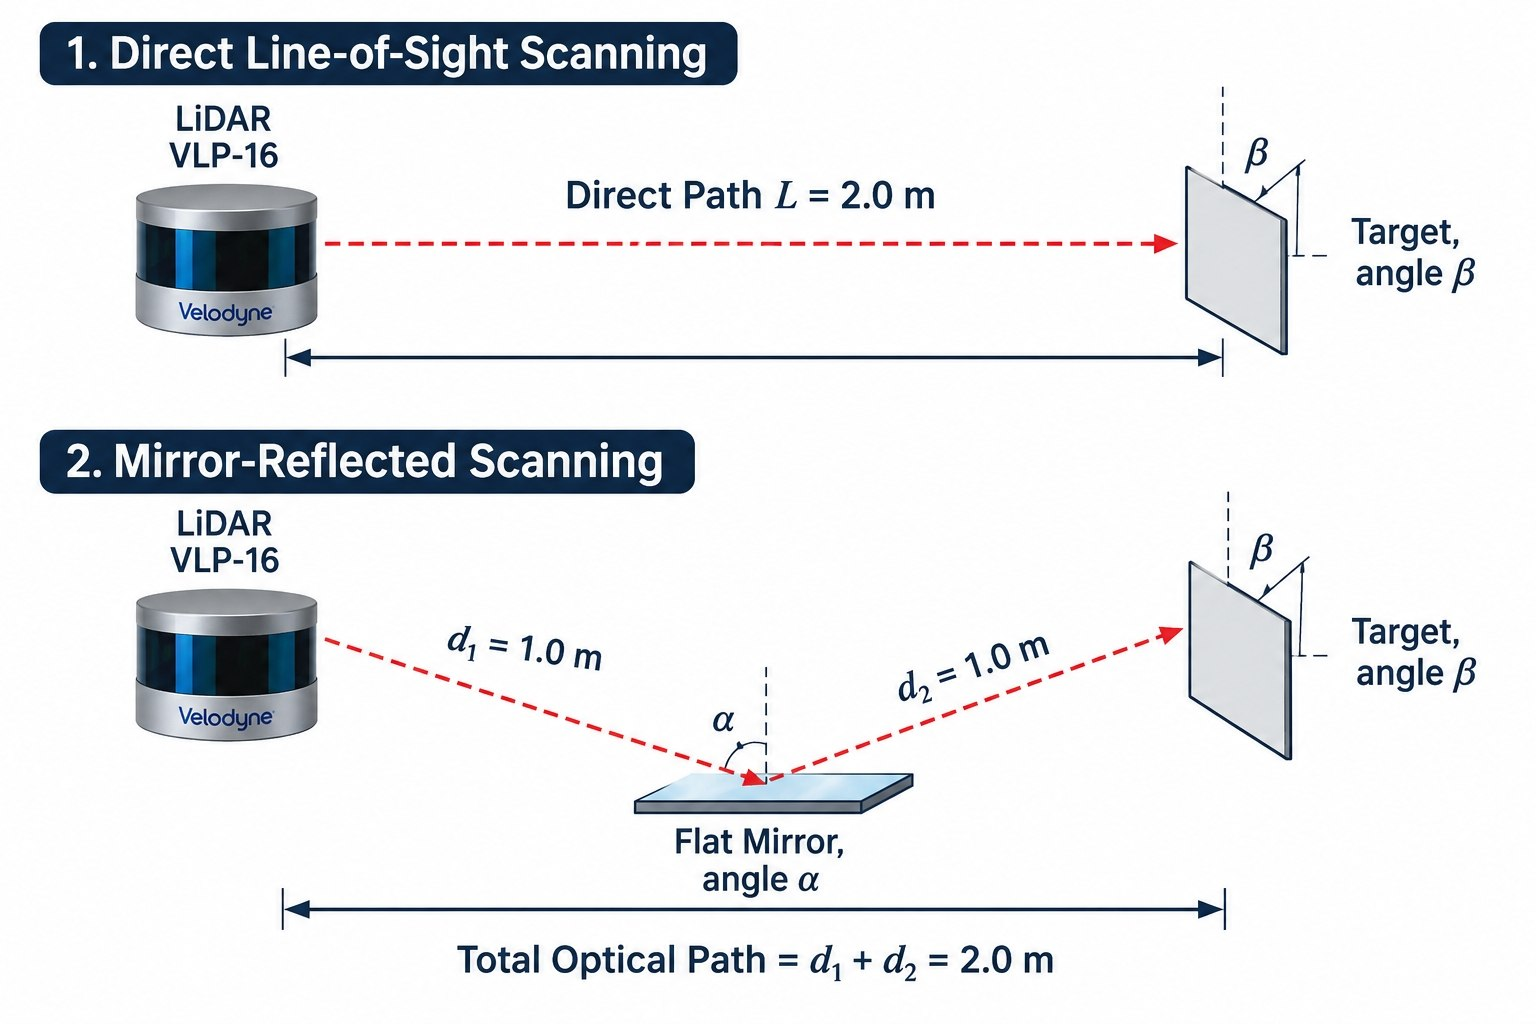
\includegraphics[width=0.95\linewidth]{images/setup_scheme.png}
\caption{Схема экспериментальной установки: 1~-- прямое сканирование ($L = 2.0$~м); 2~-- зеркально-отражённое сканирование ($d_1 + d_2 = 2.0$~м).}
\label{fig:setup}
\end{figure}

Общая длина оптического пути строго фиксируется на уровне $L_{total} = 2.0$~м ($d_1 = 1.0$~м, $d_2 = 1.0$~м). В ходе опыта независимо регулируются два угла: $\alpha$ (угол падения на зеркало) и $\beta$ (угол наклона мишени).

Запись данных выполняется в формате \texttt{.pcd} при помощи узла \texttt{mirror\_live\_node} в ROS Noetic. Сохраняются пространственные координаты точек $(X,Y,Z)$ и поле сырой интенсивности \texttt{intensity} (FLOAT32, offset=12).

На этапе постобработки облака точек выполняется пространственная сегментация плоскости мишени. Анализируются три основные метрики:

1. \textbf{Средняя интенсивность ($I_{mean}$):} Оценивается по сырым показаниям сенсора (диапазон 0--255 отсчётов):
\begin{equation}
I_{mean} = \frac{1}{N} \sum_{i=1}^{N} I_i.
\end{equation}

2. \textbf{Плотность точек ($D$):} Рассчитывается как число зарегистрированных импульсов $N$, попавших на площадь мишени $S$:
\begin{equation}
D = \frac{N}{S} \quad [\text{точек/м}^2].
\end{equation}

3. \textbf{Пространственный шум дальности (RMSE):} Для нивелирования влияния геометрии наклона $\beta$ точки мишени аппроксимируются плоскостью методом RANSAC (алгоритм SVD). Уровень шума определяется как среднеквадратичное отклонение:
\begin{equation}
RMSE = \sqrt{ \frac{1}{N} \sum_{i=1}^{N} \big( a x_i + b y_i + c z_i + d \big)^2 },
\end{equation}
где $(a,b,c,d)$~--- нормализованные параметры аппроксимированной плоскости.

Матрица пилотной серии эксперимента приведена в Таблице~\ref{tab:conditions}.

\begin{table}[htbp]
\caption{Условия проведения пилотного эксперимента ($L_{total} = 2.0$~м)}
\label{tab:conditions}
\centering
\begin{tabular}{ccccc}
\toprule
№ & Режим & $\alpha$ & $\beta$ & Описание \\
\midrule
0 & Direct & --- & $0^\circ$ & Контрольный замер (без зеркала) \\
1 & Mirror & $45^\circ$ & $0^\circ$ & Отражение под $90^\circ$ \\
2 & Mirror & $45^\circ$ & $30^\circ$ & Отражение с наклоном мишени \\
3 & Mirror & $30^\circ$ & $0^\circ$ & Острый угол падения на зеркало \\
4 & Mirror & $60^\circ$ & $0^\circ$ & Скользящий луч \\
\bottomrule
\end{tabular}
\end{table}


% ==========================================
\section{РЕЗУЛЬТАТЫ (РАЗДЕЛ НАХОДИТСЯ В СТАДИИ НАПОЛНЕНИЯ)}
% ==========================================

\textit{Примечание: физический эксперимент находится на этапе проведения. Представленные ниже рисунки \ref{fig:intensity} и \ref{fig:rmse} отражают концептуальную структуру подачи эмпирических данных и будут обновлены реальными зафиксированными значениями по завершении натурных измерений на стенде.}

\begin{figure}[htbp]
\centering
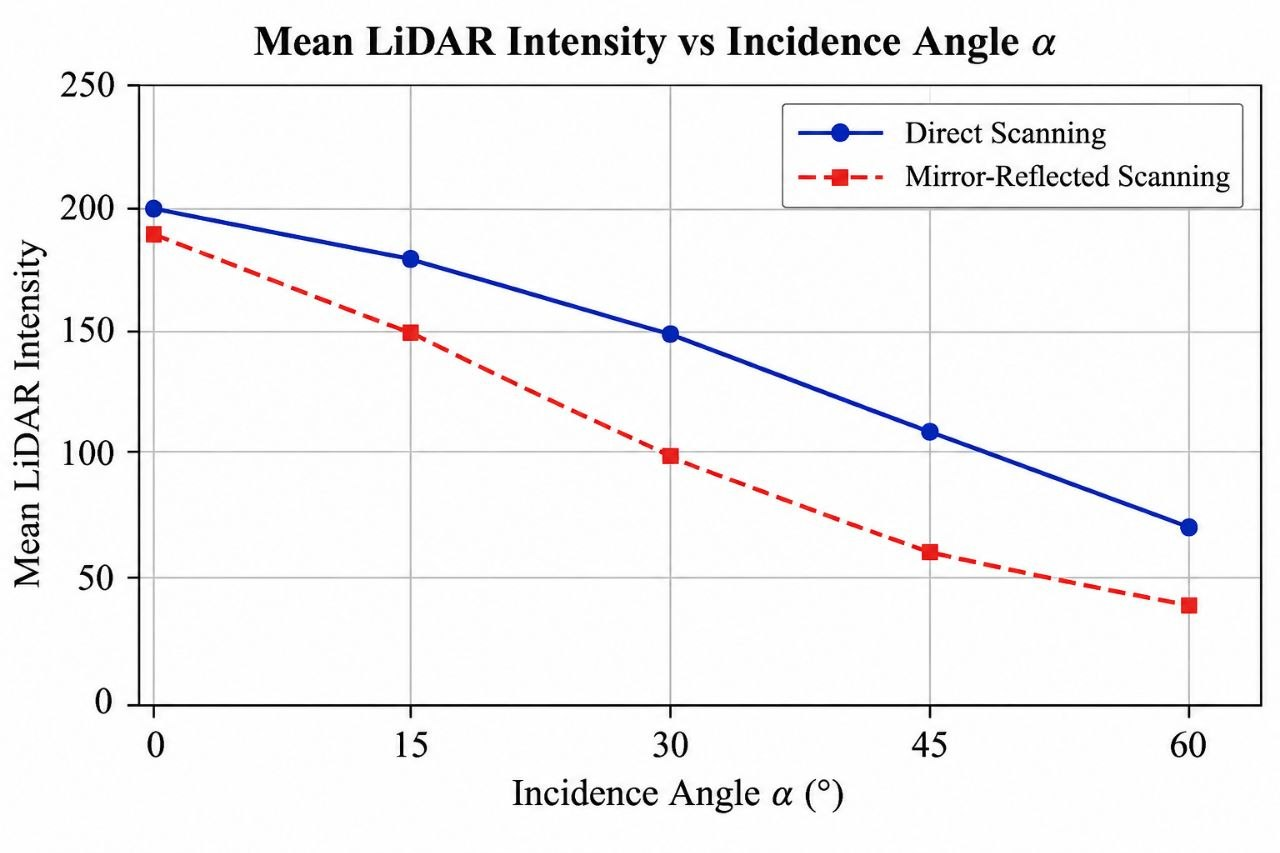
\includegraphics[width=0.95\linewidth]{images/intensity_graph.png}
\caption{Зависимость средней интенсивности $I_{mean}$ от угла падения $\alpha$ (проект макета графика; данные будут заменены по результатам натурного опыта).}
\label{fig:intensity}
\end{figure}

\begin{figure}[htbp]
\centering
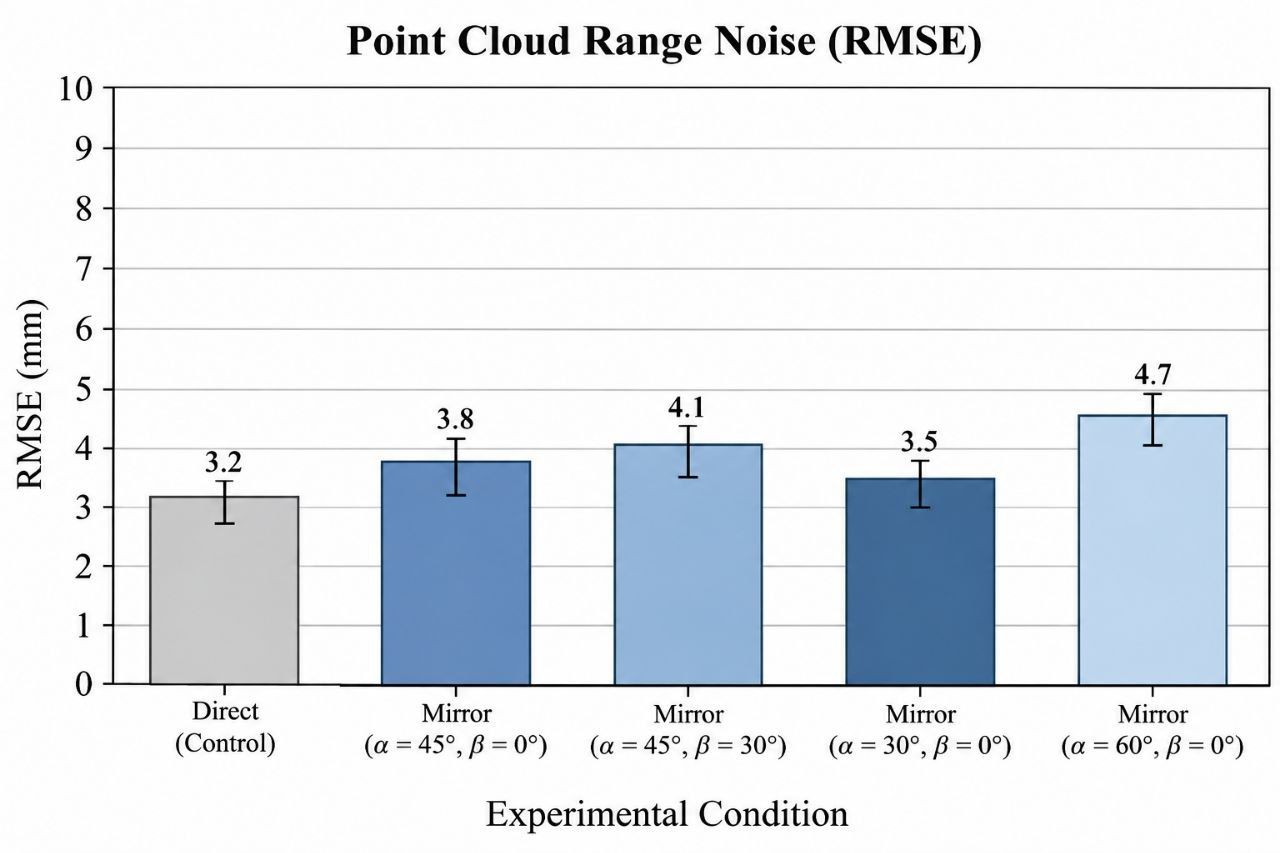
\includegraphics[width=0.95\linewidth]{images/rmse_chart.png}
\caption{Оценка пространственного шума облака точек (RMSE, мм) по условиям эксперимента (проект макета графика; данные будут заменены по результатам натурного опыта).}
\label{fig:rmse}
\end{figure}

\vspace{8cm} % Резервирование свободного места под текстовый анализ результатов после съемки data bags


% ==========================================
\section{ОБСУЖДЕНИЕ И ЗАКЛЮЧЕНИЕ}
% ==========================================

\textit{Данный раздел будет сформулирован по результатам математической обработки экспортных файлов .pcd и верификации теоретической гипотезы затухания сигналов.}

\vspace{6cm} % Резервирование места под выводы и практические рекомендации для БПЛА

% ==========================================
\begin{thebibliography}{99}

\bibitem{vishnevsky2026}
Вишневский, М.~Р., Фёдоров, И. Применение алгоритма виртуального зеркального канала LiDAR-систем с использованием автоматической калибровки // \textit{Труды Института системного программирования РАН}, 2026. Т. 38, № 3. С. 101--114.

\bibitem{soudarissanane2009}
Soudarissanane, S., et al. Influence of incidence angle on terrestrial laser scanner intensity // \textit{ISPRS}, 2009.

\bibitem{zhang2023}
Zhang, Y., et al. Radiometric characterization of Livox Mid-40 LiDAR // \textit{IEEE Transactions on Instrumentation and Measurement}, 2023.

\bibitem{li2021}
Li, F., et al. Mirror-based Extrinsic Calibration and Point Cloud Registration // \textit{IEEE Robotics and Automation Letters}, 2021.

\bibitem{soquita2025}
Soquita, R., et al. Mirror-augmented ICP SLAM for mobile robotics // \textit{Autonomous Robots}, 2025.

\bibitem{thrun2005}
Thrun, S., Burgard, W., \& Fox, D. \textit{Probabilistic robotics}. MIT press, 2005.

\bibitem{shan2018}
Shan, T., \& Englot, B. LeGO-LOAM: Lightweight and Ground-Optimized Lidar Odometry and Mapping on Variable Terrain // \textit{IEEE/RSJ International Conference on Intelligent Robots and Systems (IROS)}, 2018.

\end{thebibliography}

\end{document}
